\documentclass{article}
\usepackage{graphicx}
\usepackage{subcaption}
\usepackage{amsmath}

\begin{document}
 \begin{figure}[h]
 	\centering
 	\begin{subfigure}
 		{0,45\textwidth}
 		\centering
 		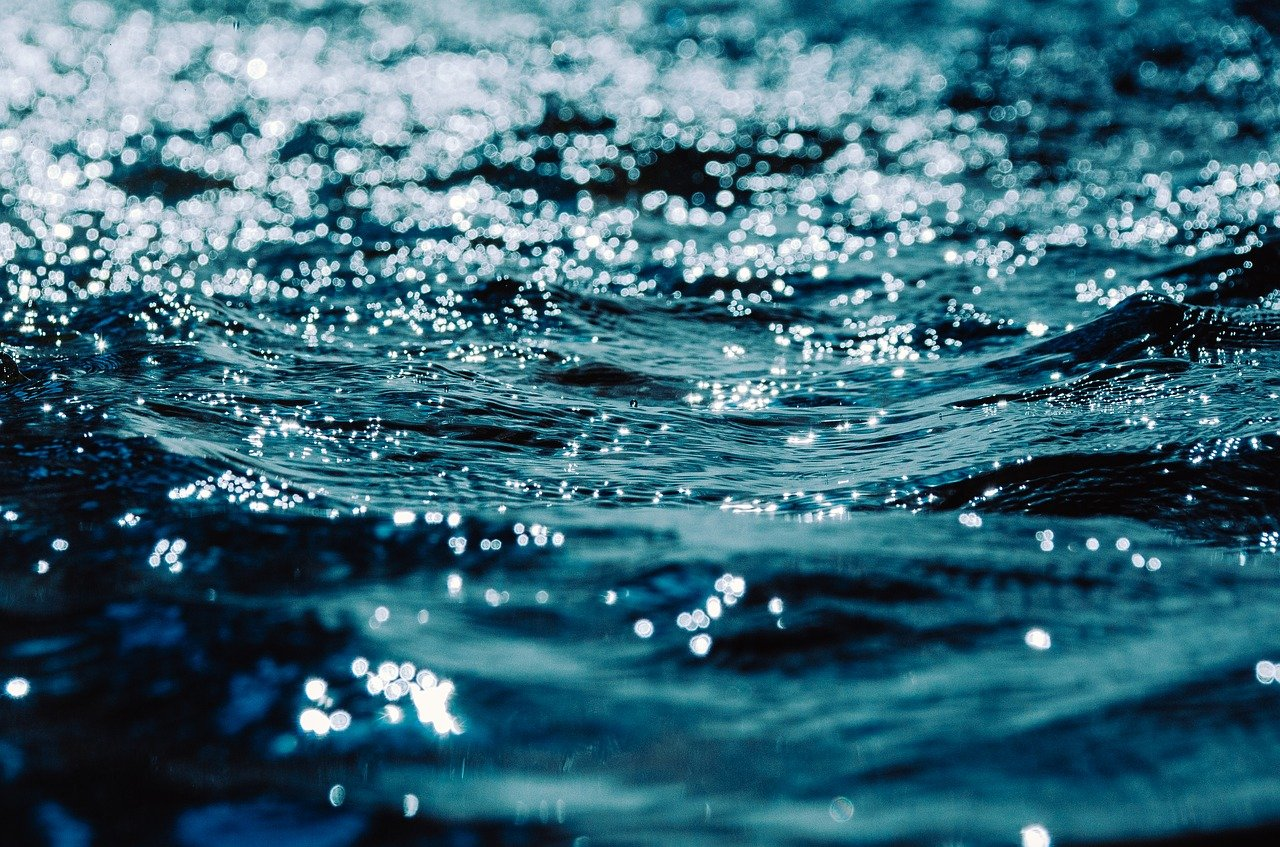
\includegraphics[width=0.9\linewidth]{img}
 		\caption{Water}
 		\label{fig:img1}
 	\end{subfigure}
 \hfill
    \begin{subfigure}{0.45\textwidth}
    	
\includegraphics[width=0.9\linewidth]{img2}
    	\caption{img2}
    	\label{fig:img2}
    	
    \end{subfigure}
   \caption{Side by Side Images}
 \end{figure}
	\[x^2 + x + c\]\
	\[a^2 + 2ab + b^2\]\
	\begin{equation}
		a^2 + b^2 + 2ab = (a+b)^2 
	\end{equation}
    This is a simple math expression \[\sqrt{a+b}\]\
    \begin{align}
    	f(x) & = x^2 \\
    	g(x) & = \frac{1}{x} \\
    	F(x) & = \int_{a}^{b}{e^{t^2}}
    \end{align}
\end{document}